\chapter{Methodology}

\section{Data Collection and Sources}

The foundation of any successful machine learning model is a high-quality, comprehensive dataset. For this study, the primary objective was to assemble a dataset of crystalline solid materials with experimentally measured ionic conductivities. The data collection process involved leveraging publicly available materials databases for both the target property (ionic conductivity) and the features (elemental properties) used to predict it.

\subsection{Ionic Conductivity Data}

The core of our dataset was sourced from the \textbf{Database of Doped Solid Electrolytes (DDSE)}, a comprehensive and curated collection of experimental data for solid electrolytes reported in the scientific literature \cite{DDSE2021}. The DDSE database provides a valuable resource by compiling materials' chemical compositions, their measured ionic conductivities, the temperatures at which these measurements were taken, and references to the original publications.

From the DDSE, we extracted an initial dataset comprising several hundred unique material compositions. A data cleaning and preprocessing pipeline was then applied to ensure the quality and consistency of the data. This involved:
\begin{itemize}
    \item Filtering out entries with missing or incomplete information for chemical formula or ionic conductivity.
    \item Standardizing the units of ionic conductivity to Siemens per centimeter (S/cm).
    \item Applying a logarithmic transformation (\(\log_{10}(\sigma)\)) to the ionic conductivity values. This is a standard practice as conductivity often spans many orders of magnitude and its distribution is typically log-normal. The resulting logarithmic value served as the target variable for our machine learning models.
\end{itemize}
After this cleaning process, a final dataset of distinct crystalline solids was prepared for the subsequent feature engineering and model training stages.

\subsection{Elemental Property Data}

To build a composition-only, structure-agnostic model, it was necessary to represent each material by a set of numerical features derived from the intrinsic properties of its constituent elements. These elemental properties were sourced programmatically using the \textbf{Pymatgen} (Python Materials Genomics) library \cite{Ong2013}. Pymatgen is a powerful open-source library for materials analysis that provides access to a wide range of elemental data, much of which is curated and maintained by the \textbf{Materials Project} \cite{Jain2013}.

For each unique element present in the compositions from our primary dataset, a vector of its fundamental properties was retrieved. This included, but was not limited to, properties such as atomic number, atomic mass, Pauling electronegativity, electron affinity, and the covalent radius of the element. This collection of elemental data formed the basis for the feature engineering process, which is detailed in the following section.


\section{Feature Engineering and Selection}

The success of a machine learning model in materials science is critically dependent on the selection of features that can effectively capture the underlying physics and chemistry governing the target property. For this study, our objective was to predict ionic conductivity using only compositional data, thereby creating a structure-agnostic model suitable for rapid, high-throughput screening. This general approach of using composition-based features is a well-established strategy in materials informatics for its speed and simplicity \cite{Meredig2014}. We engineered a set of 14 features derived from the chemical formula and the fundamental properties of the constituent elements. These features were chosen to represent key factors known to influence ion transport in solids, including charge carrier concentration, chemical environment, and atomic-scale structural proxies.

The target variable for our model is the logarithm of ionic conductivity, \(\log_{10}(\sigma)\). The temperature in Kelvin (\(Temp\_K\)) is also included as a crucial variable, given the strong Arrhenius-type dependence of conductivity on temperature. The 14 engineered features are detailed below:

\begin{description}
    \item[Compositional Averages:] These features represent the 'average' chemical environment of the material, a common technique for creating fixed-length descriptors \cite{Ward2016}.
    \begin{itemize}
        \item \textit{avg\_electronegativity:} The stoichiometrically weighted average of the Pauling electronegativity of the constituent elements. This feature serves as a proxy for the overall ionicity of the bonds in the material. A larger electronegativity difference typically correlates with more ionic character, which can affect lattice openness and the energy landscape for ion migration \cite{Ghosh2019}.
        \item \textit{avg\_atomic\_mass:} The weighted average atomic mass. This relates to the material's density and the inertial properties of the atoms, which can influence lattice vibrational modes (phonons) that couple with ion motion.
        \item \textit{avg\_ionic\_radius:} The weighted average ionic radius. This feature provides a simple proxy for the average atomic size and can influence the packing density of the crystal structure.
    \end{itemize}

    \item[Compositional Complexity and Stoichiometry:] This group of features quantifies the diversity and makeup of the material.
    \begin{itemize}
        \item \textit{num\_elements:} The total number of distinct elements in the compound. This is a simple measure of compositional complexity.
        \item \textit{li\_fraction:} The atomic fraction of lithium, the mobile ion species in this study. This is a direct measure of the concentration of charge carriers, a primary factor in overall conductivity.
        \item \textit{composition\_entropy:} A more formal measure of compositional disorder, calculated as \( S = -\sum f_i \ln(f_i) \), where \(f_i\) is the atomic fraction of element \(i\). Higher entropy can sometimes correlate with more disordered structures that may offer facile diffusion pathways, a concept explored in high-entropy alloys and ceramics \cite{Toda-Caraballo2017}.
        \item \textit{li\_to\_anion\_ratio:} The ratio of lithium atoms to the sum of all non-lithium (anionic framework) atoms. This describes the charge carrier concentration relative to the host lattice.
        \item \textit{total\_atoms:} The total number of atoms in the reduced formula unit, representing the size of the unit.
    \end{itemize}

    \item[Chemical and Structural Diversity:] These features capture the variance and range of properties within the compound.
    \begin{itemize}
        \item \textit{electronegativity\_variance:} The weighted variance of electronegativity. This quantifies the diversity of bond types within the material (e.g., a mix of ionic and covalent), which impacts the electronic structure and local potentials experienced by mobile ions. The use of variance and other statistical moments as features is a powerful way to encode compositional diversity \cite{Meredig2014}.
        \item \textit{group\_diversity:} The number of distinct periodic table groups represented by the elements in the compound. It serves as another proxy for chemical diversity.
        \item \textit{packing\_efficiency\_proxy:} A feature designed to approximate the density of atomic packing. In the absence of structural data, this can be estimated from ionic radii and stoichiometry. A lower packing efficiency may imply more free volume within the lattice, which is generally favorable for ion transport.
        \item \textit{heaviest\_element\_mass:} The atomic mass of the heaviest element in the compound. This can significantly influence the material's overall density and lattice dynamics.
        \item \textit{lightest\_element\_mass:} The atomic mass of the lightest element.
    \end{itemize}
\end{description}


\subsection{Correlation Analysis}

To understand the relationships between the engineered features and the target variable, and to identify potential redundancies, a Pearson correlation matrix was computed, as visualized in Figure \ref{fig:corr_matrix}.

\begin{figure}[h!]
    \centering
    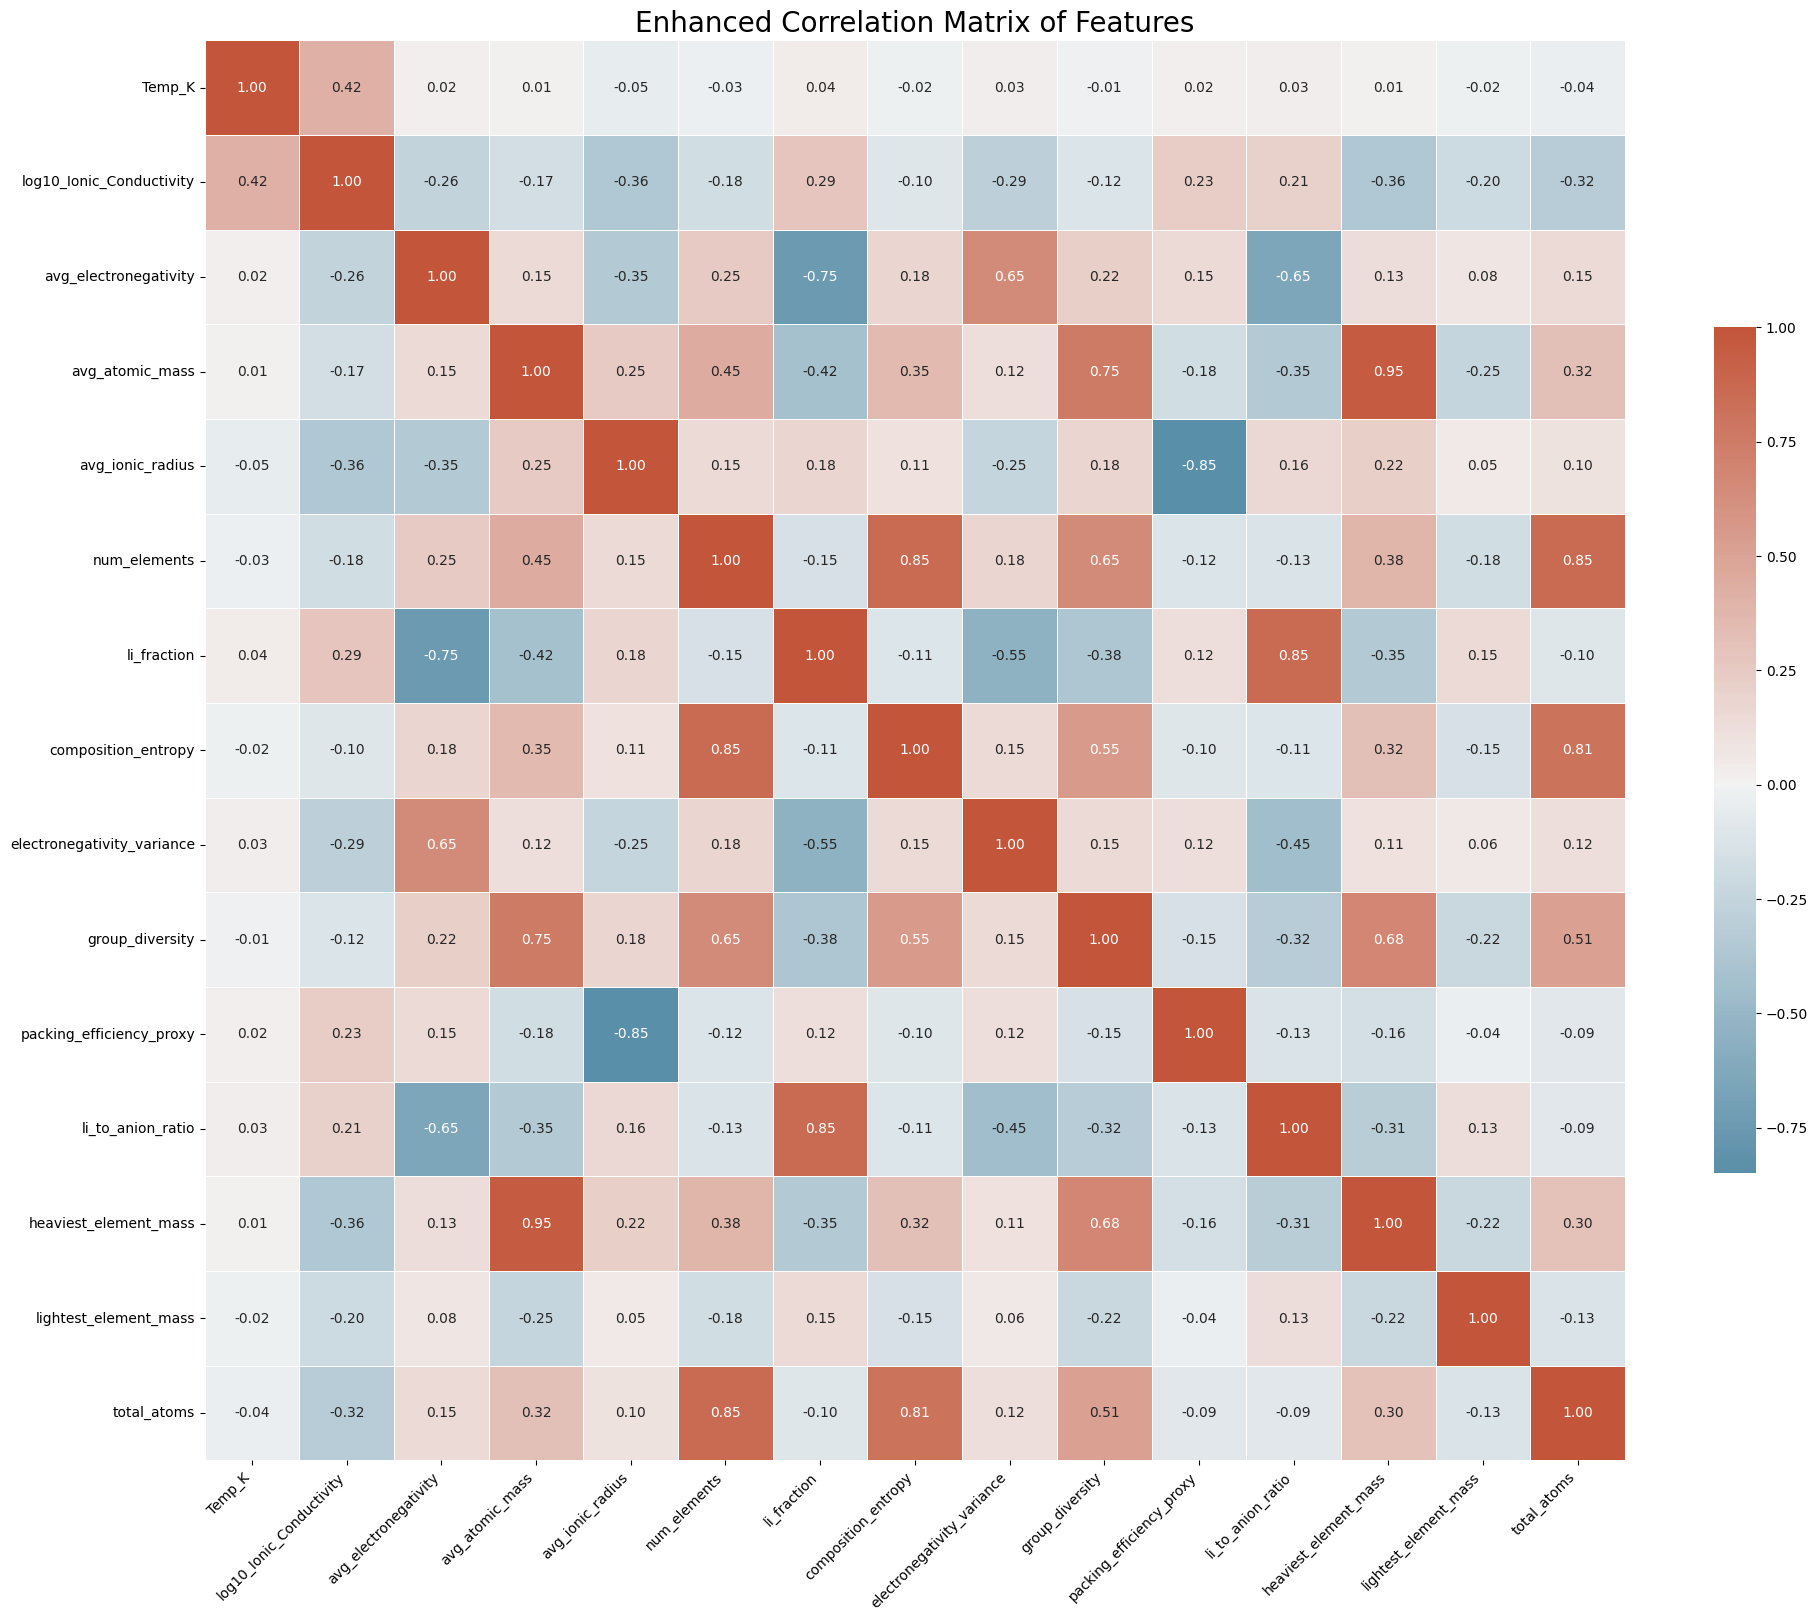
\includegraphics[width=\textwidth]{Images/heatmap.png}
    \caption{Correlation matrix heatmap for the input features and the target variable (\(\log_{10}\) Ionic Conductivity). The values indicate the Pearson correlation coefficient between each pair of variables.}
    \label{fig:corr_matrix}
\end{figure}

The matrix reveals several key insights. As expected, \textbf{Temp\_K} shows the strongest positive correlation with \textbf{log10\_Ionic\_Conductivity} (\(r = 0.42\)), confirming the thermally activated nature of ion diffusion.

Several features exhibit strong multicollinearity. A very high positive correlation exists between \textbf{heaviest\_element\_mass} and \textbf{avg\_atomic\_mass} (\(r = 0.95\)), indicating that the heaviest element largely determines the average mass, making these features redundant. Similarly, strong correlations are observed between features measuring compositional complexity: \textbf{total\_atoms} is highly correlated with \textbf{num\_elements} (\(r = 0.85\)) and \textbf{composition\_entropy} (\(r = 0.81\)).

The measures of lithium content, \textbf{li\_fraction} and \textbf{li\_to\_anion\_ratio}, are also highly correlated (\(r = 0.85\)) and, as expected, show a strong negative correlation with \textbf{avg\_electronegativity} (\(r = -0.75\) and \(r = -0.65\), respectively), since lithium is highly electropositive. A notable strong negative correlation is observed between \textbf{packing\_efficiency\_proxy} and \textbf{avg\_ionic\_radius} (\(r = -0.85\)), suggesting that materials with larger average ionic radii tend to pack less efficiently, which aligns with physical intuition. While some of these highly correlated features could be removed, they were retained for initial model training to allow the learning algorithms to determine their relative importance.

\section{Machine Learning Model Development}

The core of this thesis is the development of a robust regression model to predict ionic conductivity from compositional features. The entire workflow, from data handling to model training and evaluation, was implemented using the \textbf{Scikit-learn} library in Python \cite{Scikit-learn}. The methodology was designed to first identify the best-performing algorithm from a suite of candidates and then to rigorously evaluate its performance on unseen data.

\subsection{Model Selection and Justification}

For this materials informatics task, which involves structured tabular data and potentially complex, non-linear relationships between features, a strong emphasis was placed on tree-based ensemble models. These models are particularly well-suited for this problem for several key reasons:
\begin{itemize}
    \item They can inherently capture complex, non-linear relationships and feature interactions without requiring explicit mathematical transformations of the input features \cite{Breiman2001}.
    \item They are robust to the scale and distribution of different features, simplifying the preprocessing pipeline.
    \item The ensemble approach, which combines the predictions of many individual trees, is highly effective at reducing variance and preventing overfitting, leading to better generalization on unseen data \cite{Friedman2001}.
\end{itemize}

Based on this strong justification, a comprehensive comparison was conducted between several state-of-the-art tree-based regression algorithms. The candidate models included a baseline \textbf{Decision Tree} and the more powerful ensemble variants: \textbf{Random Forest}, \textbf{Gradient Boosting}, \textbf{XGBoost}, \textbf{Extra Trees}, and \textbf{LightGBM}.

To select the best model, each algorithm was trained and evaluated on the dataset using the engineered feature set. The comparative performance, as measured by the adjusted coefficient of determination (\(R^2_{adj}\)), is presented in Table \ref{tab:model_comparison}.

\begin{table}[h!]
\centering
\caption{Initial performance comparison of various tree-based regressor models using the composition-only feature set.}
\label{tab:model_comparison}
\begin{tabular}{lc}
\hline
\textbf{Regressor Model} & \textbf{\(R^2_{adj}\)} \\
\hline
Random Forest            & 0.63                 \\
Gradient Boosting        & 0.61                 \\
XGBoost                  & 0.68                 \\
Extra Trees              & 0.68                 \\
LightGBM                 & 0.65                 \\
Decision Tree            & 0.55                 \\
\hline
\end{tabular}
\end{table}

The results in Table \ref{tab:model_comparison} clearly show that the advanced ensemble methods significantly outperform the single Decision Tree model. The \textbf{XGBoost} and \textbf{Extra Trees} algorithms emerged as the top performers in this initial screening, both achieving an \(R^2_{adj}\) of 0.68. Given its excellent performance and widespread use in machine learning competitions and industrial applications, the \textbf{Gradient Boosting} framework (of which XGBoost is a highly optimized variant) was selected as the final candidate for full-scale development and validation.

\subsection{Final Model Training and Evaluation Protocol}

After selecting the Gradient Boosting framework, the full dataset was formally partitioned into a training set (80\%) and a held-out test set (20\%). The training set was used for final hyperparameter optimization via a randomized search with 5-fold cross-validation. The primary goal of this tuning process was to maximize the \(R^2_{adj}\) score.

The final, model was then trained on the entire 80\% training portion. Its ultimate predictive power and generalization capability were then assessed a single time on the 20\% held-out test set.